\documentclass[main.tex]{subfiles}

% Load any packages needed for this document
\begin{document}
%-------------------------------------------------------------------------------------------%
<p>
\section{Regression Diagnostics with \texttt{R} }
% http://www.statmethods.net/stats/rdiagnostics.html

<p>
\section{Diagnostic Plots for Linear Models with \texttt{R}}
Plot Diagnostics for an \texttt{lm} Object



#### Description}

Six plots (selectable by \texttt{which}) are currently available: 
\begin{enumerate}
* a plot of residuals against fitted values, 
* a Scale-Location plot of \textit{sqrt(| residuals |}) against fitted values, 
* a Normal Q-Q plot, 
* a plot of Cook's distances versus row labels, 
* a plot of residuals against leverages, 
* a plot of Cook's distances against leverage/(1-leverage).
\end{enumerate} By default, the first three and 5 are provided.


* The \textbf{Scale-Location} plot, also called ‘Spread-Location’ or ‘S-L’ plot, takes the square root of the absolute residuals in order to diminish skewness (sqrt(|E|)) is much less skewed than | E | for Gaussian zero-mean E).

* The \textbf{Residual-Leverage} plot shows contours of equal Cook's distance, for values of cook.levels (by default 0.5 and 1) and omits cases with leverage one with a warning. If the leverages are constant (as is typically the case in a balanced aov situation) the plot uses factor level combinations instead of the leverages for the x-axis. (The factor levels are ordered by mean fitted value.)


```{r}
par(mfrow=c(4,1))
plot(fittedmodel)
par(opar)

<p>
%http://stats.stackexchange.com/questions/58141/interpreting-plot-lm
 I explained the assumption of homoscedasticity and the plots that can help you assess it (including scale-location plots [2]) on CV here: What does having constant variance in a linear regression model mean? I have discussed qq-plots [3] on CV here: QQ plot does not match histogram. So, what's left is primarily just understanding [5], the residual-leverage plot.

To understand this, we need to understand three things:


* leverage,
* standardized residuals, and
* Cook's distance.

%%%%%%%%%%%%%%%%%%%%%%%%%%%%%%%%%%%%%%%%%

\subsection{Diagnostic Plots for LMs}
%-------------------------------------------------------------------------------------------%

\item
The \textbf{Scale-Location} plot, also called ‘Spread-Location’ (or ‘S-L’ plot), takes the square root of the absolute residuals in order to diminish skewness (sqrt($|E|)$) is much less skewed than $| E |$ for Gaussian zero-mean E).

\item
The \textbf{Residual-Leverage} plot shows contours of equal Cook's distance, for values of \texttt{cook.levels} (by default 0.5 and 1) and omits cases with leverage one with a warning. If the leverages are constant (as is typically the case in a balanced aov situation) the plot uses factor level combinations instead of the leverages for the x-axis. \\
\textit{(The factor levels are ordered by mean fitted value.)}

\begin{framed}
\begin{verbatim}
plot(lm(mpg~wt+cyl),which=c(1),pch=18,col="red")
plot(lm(mpg~wt+cyl),which=c(2),pch=18,col="red")
plot(lm(mpg~wt+cyl),which=c(3),pch=18,col="red")
plot(lm(mpg~wt+cyl),which=c(4),pch=18,col="red")
plot(lm(mpg~wt+cyl),which=c(5),pch=18,col="red")
plot(lm(mpg~wt+cyl),which=c(6),pch=18,col="red")
\end{verbatim}
\end{framed}

\begin{figure}[h!]
\centering
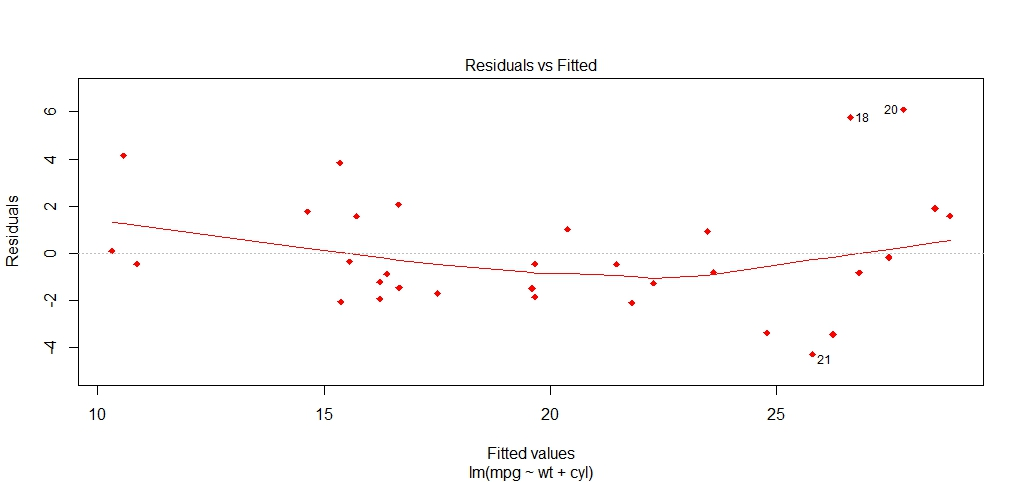
\includegraphics[width=0.9\linewidth]{./mtcarsDiagPlot1}

\label{mtcarsDiagPlot1}
\end{figure}

<p>
\begin{figure}[h!]
\centering
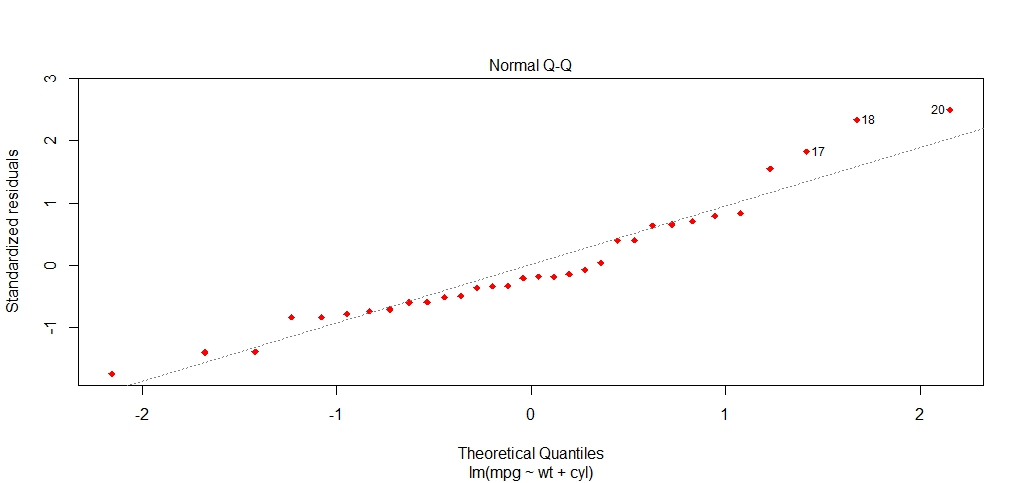
\includegraphics[width=0.9\linewidth]{./mtcarsDiagPlot2}

\label{mtcarsDiagPlot2}
\end{figure}

\subsubsection{Plot 3 : Normal Probability Plot}
This plot is used to assess the validity of the normality of the residuals.
\begin{figure}[h!]
\centering
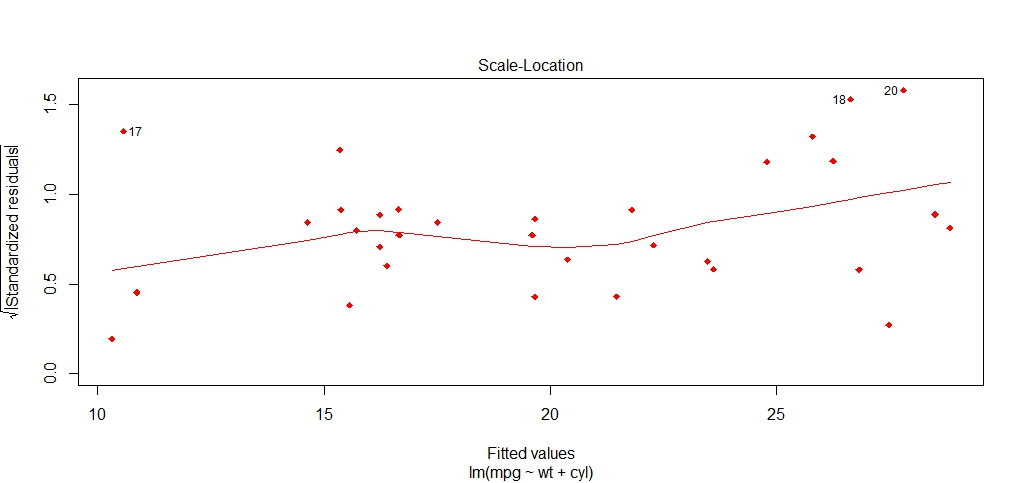
\includegraphics[width=0.9\linewidth]{./mtcarsDiagPlot3}

\label{mtcarsDiagPlot3}
\end{figure}

<p>
\subsubsection{Plot 5 :  Cook's Distance}
\begin{figure}[h!]
\centering
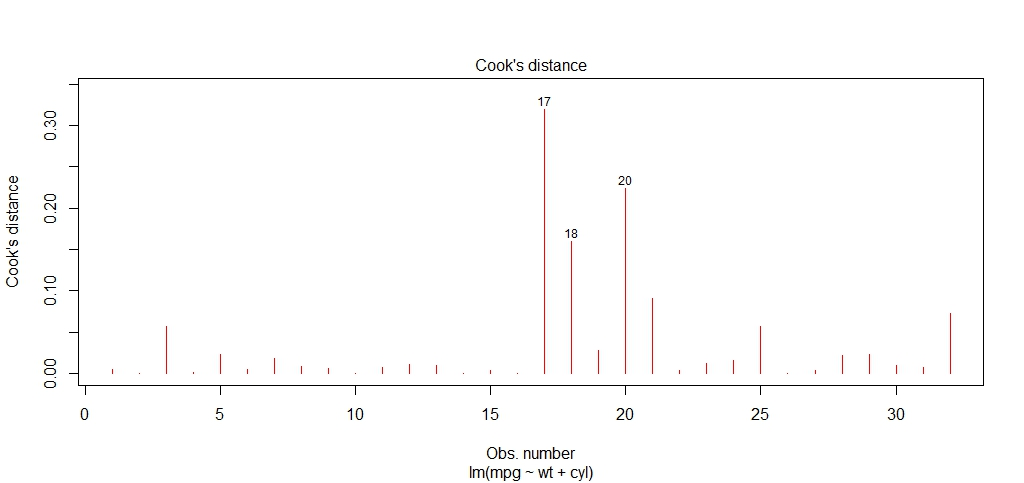
\includegraphics[width=0.9\linewidth]{./mtcarsDiagPlot4}

\label{mtcarsDiagPlot4}
\end{figure}


\begin{figure}[h!]
\centering
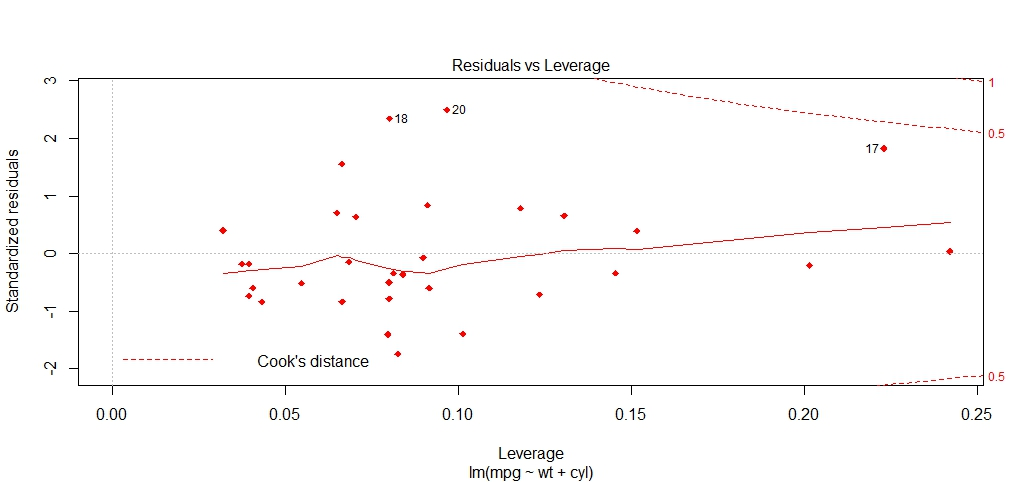
\includegraphics[width=0.9\linewidth]{./mtcarsDiagPlot5}

\label{mtcarsDiagPlot5}
\end{figure}


\subsubsection{Plot 6 :  Cook's Distance vs Leverage}
\begin{figure}[h!]
\centering
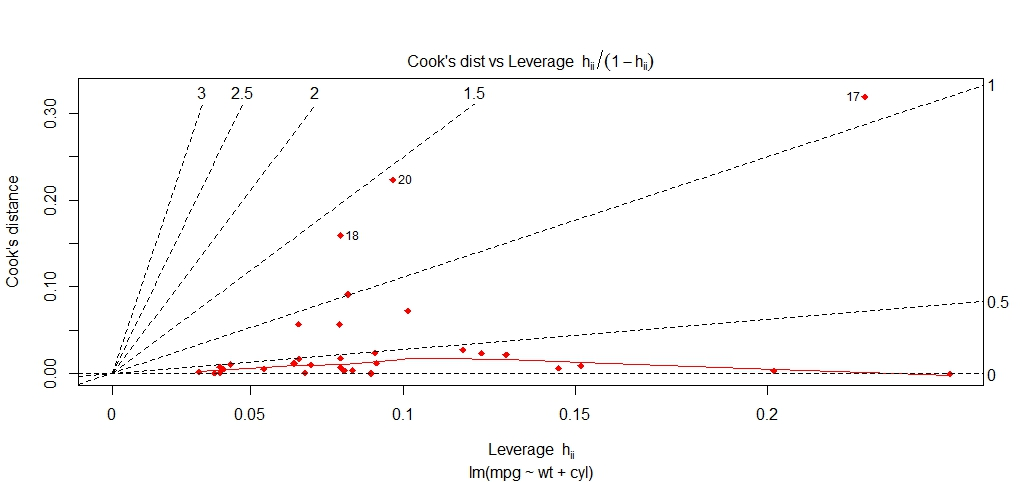
\includegraphics[width=0.9\linewidth]{./mtcarsDiagPlot6}

\label{mtcarsDiagPlot6}
\end{figure}


\begin{framed}
\begin{verbatim}
par(mfrow=c(4,1))
plot(fittedmodel)
par(opar)
\end{verbatim}
\end{framed}

% http://www.columbia.edu/~cjd11/charles_dimaggio/DIRE/resources/R/rFunctionsList.pdf

\end{document}
